\section{Results}\label{sec:results}

Muons and neutrons were produced by the electron beam interaction with the beam-dump and propagated in the region of interest as described in  Sec.~\ref{sec:sampling}.


\subsubsection{Muons}
Fig.~\ref{fig:mu-comp} shows the muon flux  as obtained by GEMC and FLUKA starting from the electron/beam-dump interaction and as generated at high statistics by the custom muon generator in the  three locations of interest. Results are reported for muons generated at high statistic by the custom $\mu$ event generator and propagated using GEMC (green points in the figure).
The number of event generating at the dump correspond to  (1.2 $\pm$0.1) 10$^{12}$ EOT that correspond to a  0.2 uA 
\begin{figure}[h!] 
\center
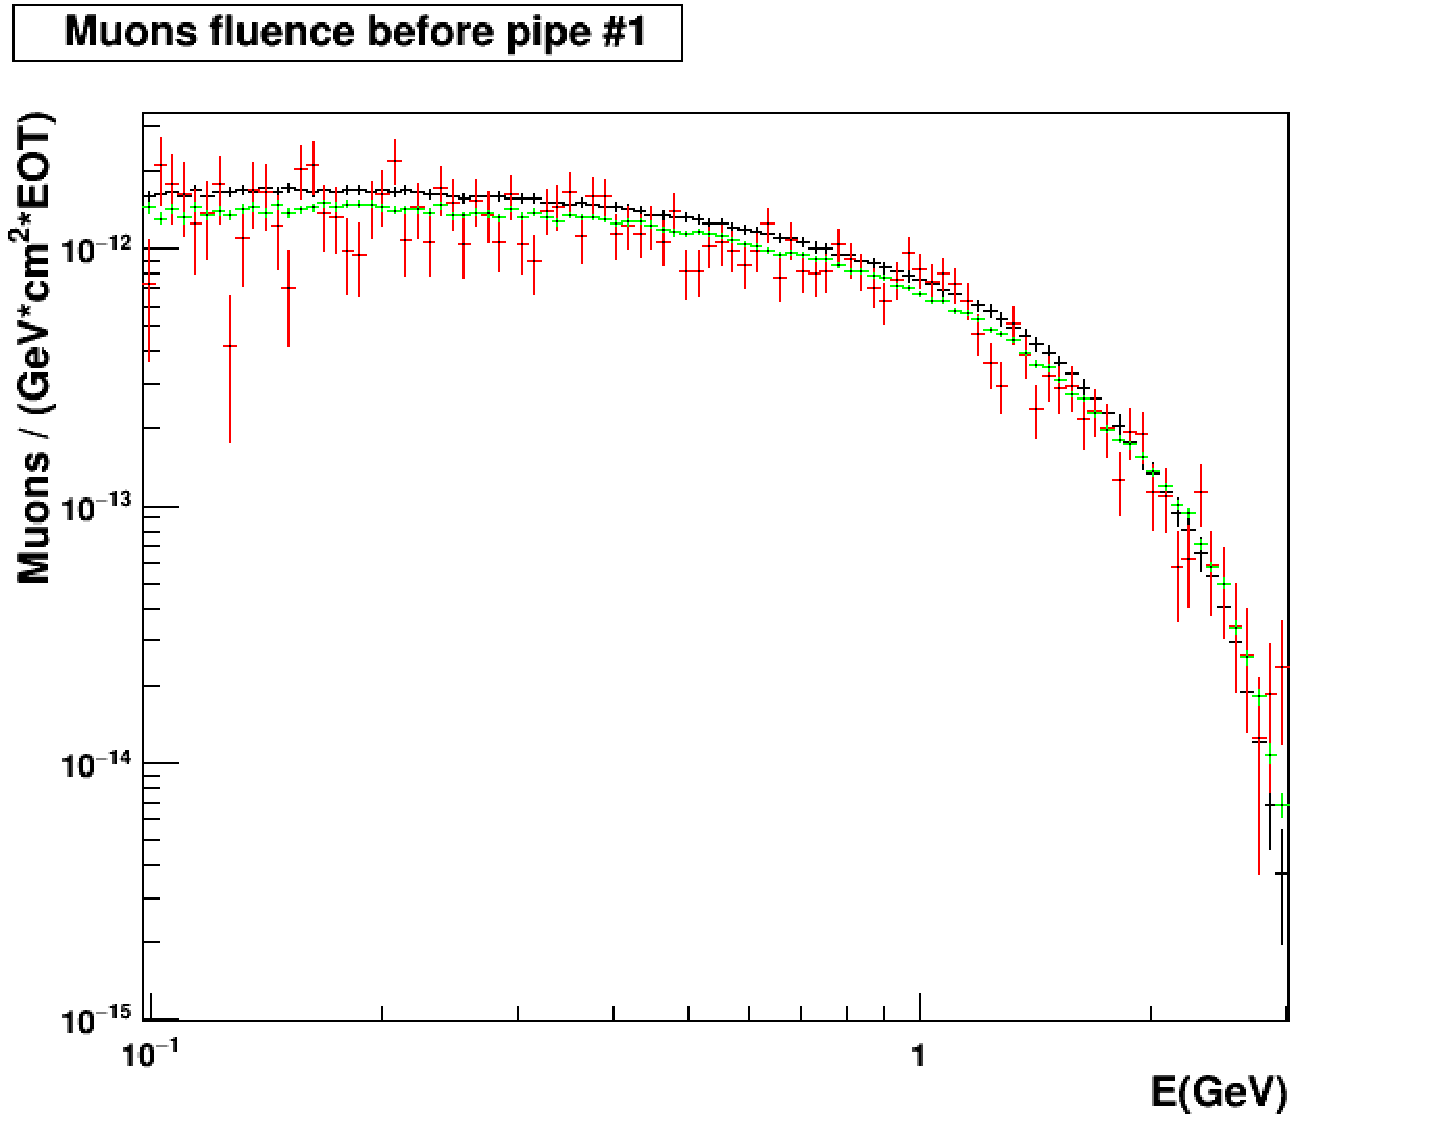
\includegraphics[width=4.7cm]{figs/comparisonMuonsPipe1_1D.pdf}
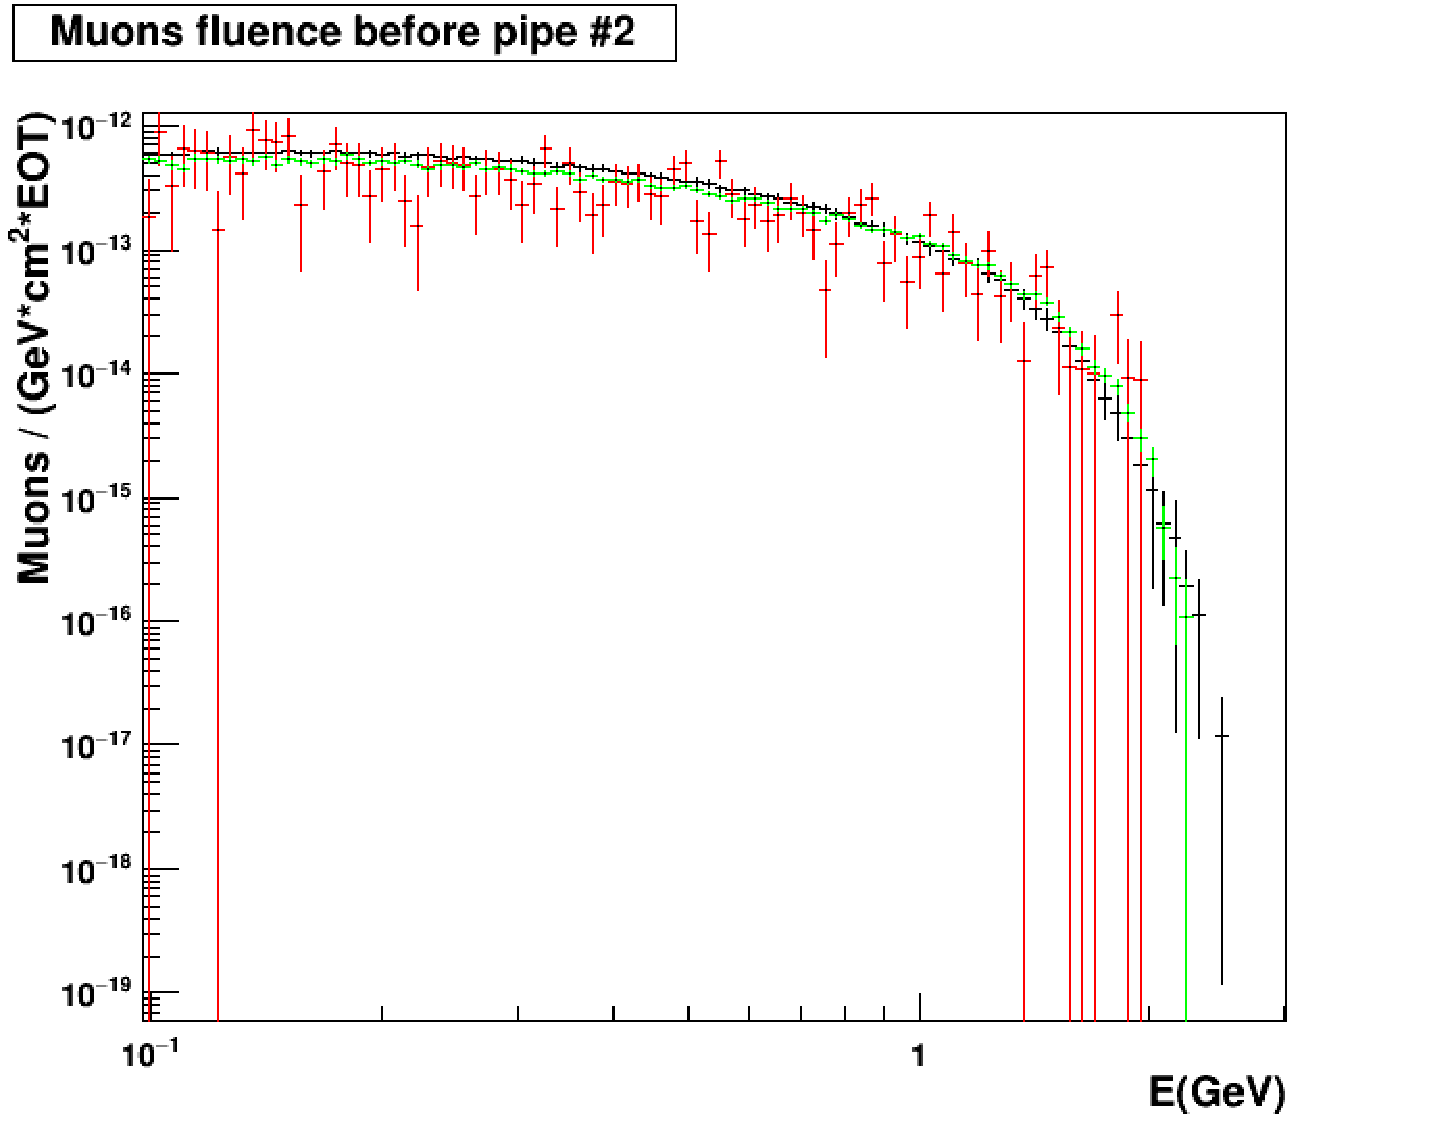
\includegraphics[width=4.7cm]{figs/comparisonMuonsPipe2_1D.pdf}
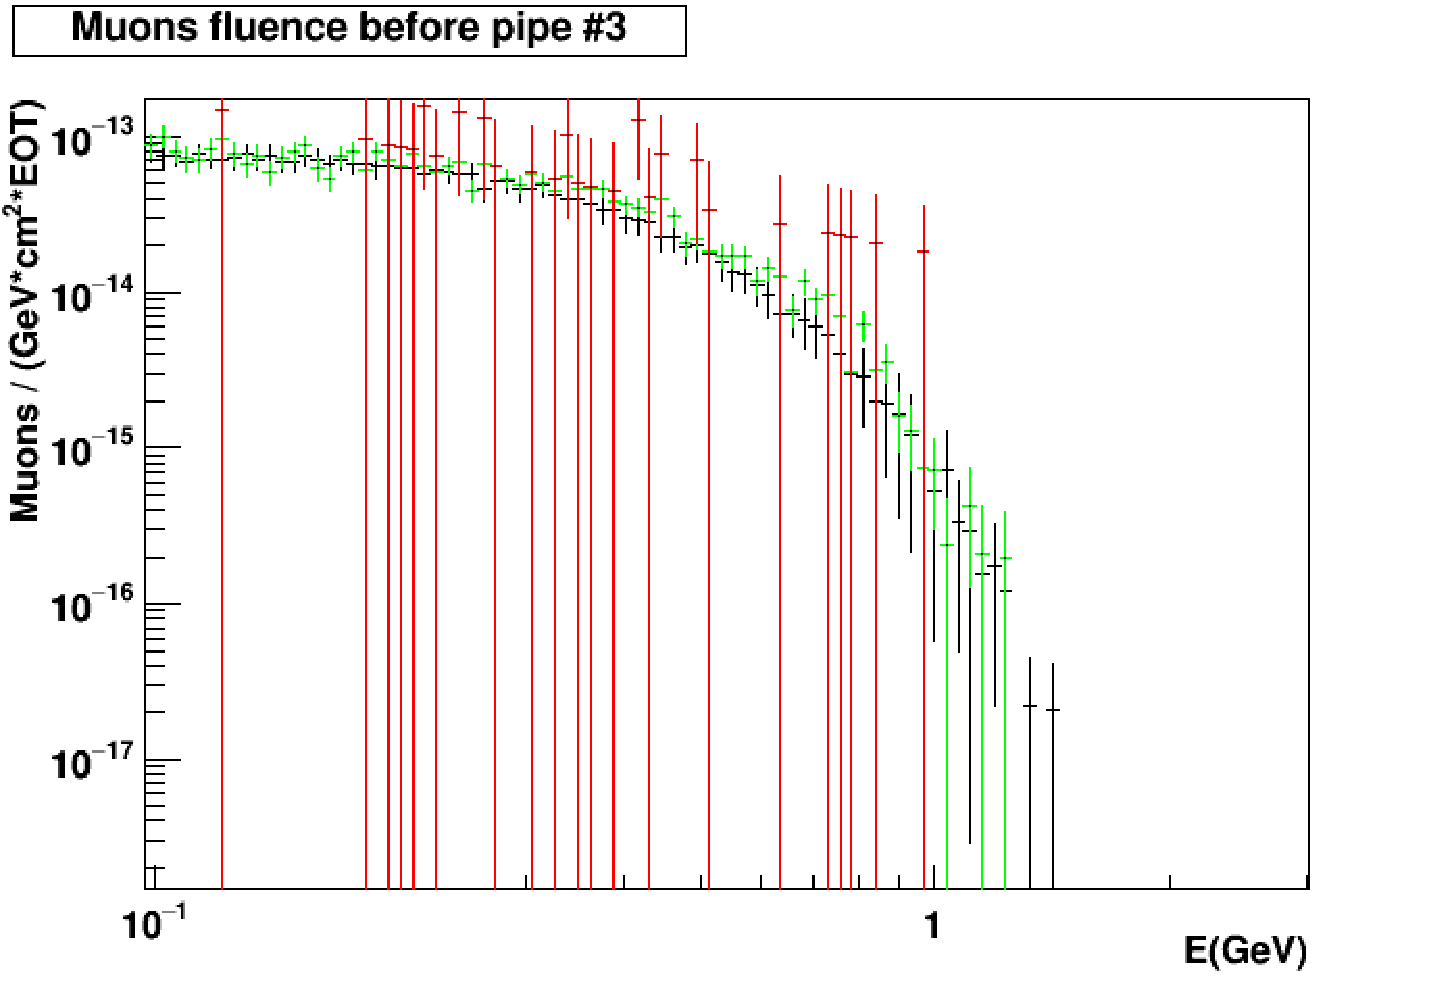
\includegraphics[width=5.5cm]{figs/comparisonMuonsPipe3_1D.pdf}
\caption{Muons energy spectra at the three locations of interest. Beam/dump interaction using  FLUKA (black), GEMC (red) and the high statistic custom $\mu$ event generator with GEMC propagation (green).}
\label{fig:mu-comp}
\end{figure}
\subsubsection{Beam-related background}



Fig.~\ref{fig:nu-comp} shows the neutron flux  as obtained by  FLUKA starting from the electron/beam-dump interaction  in the  three locations of interest. 
\begin{figure}[h!] 
\center
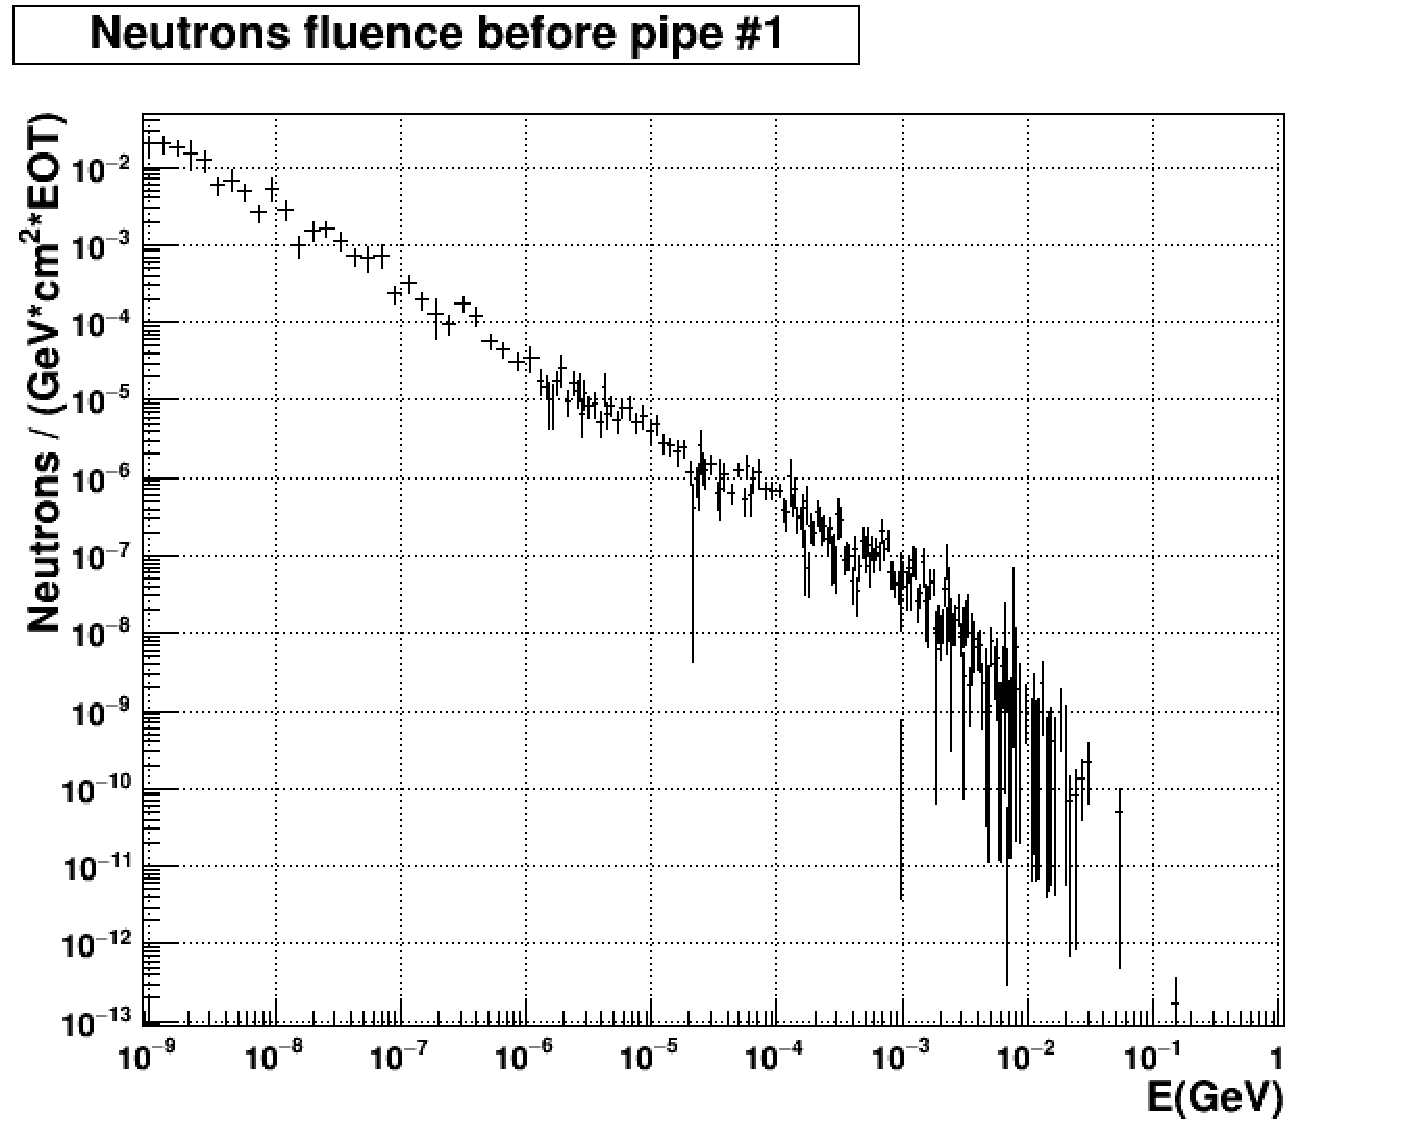
\includegraphics[width=4.7cm]{figs/NeutronsPipe1_1D.pdf}
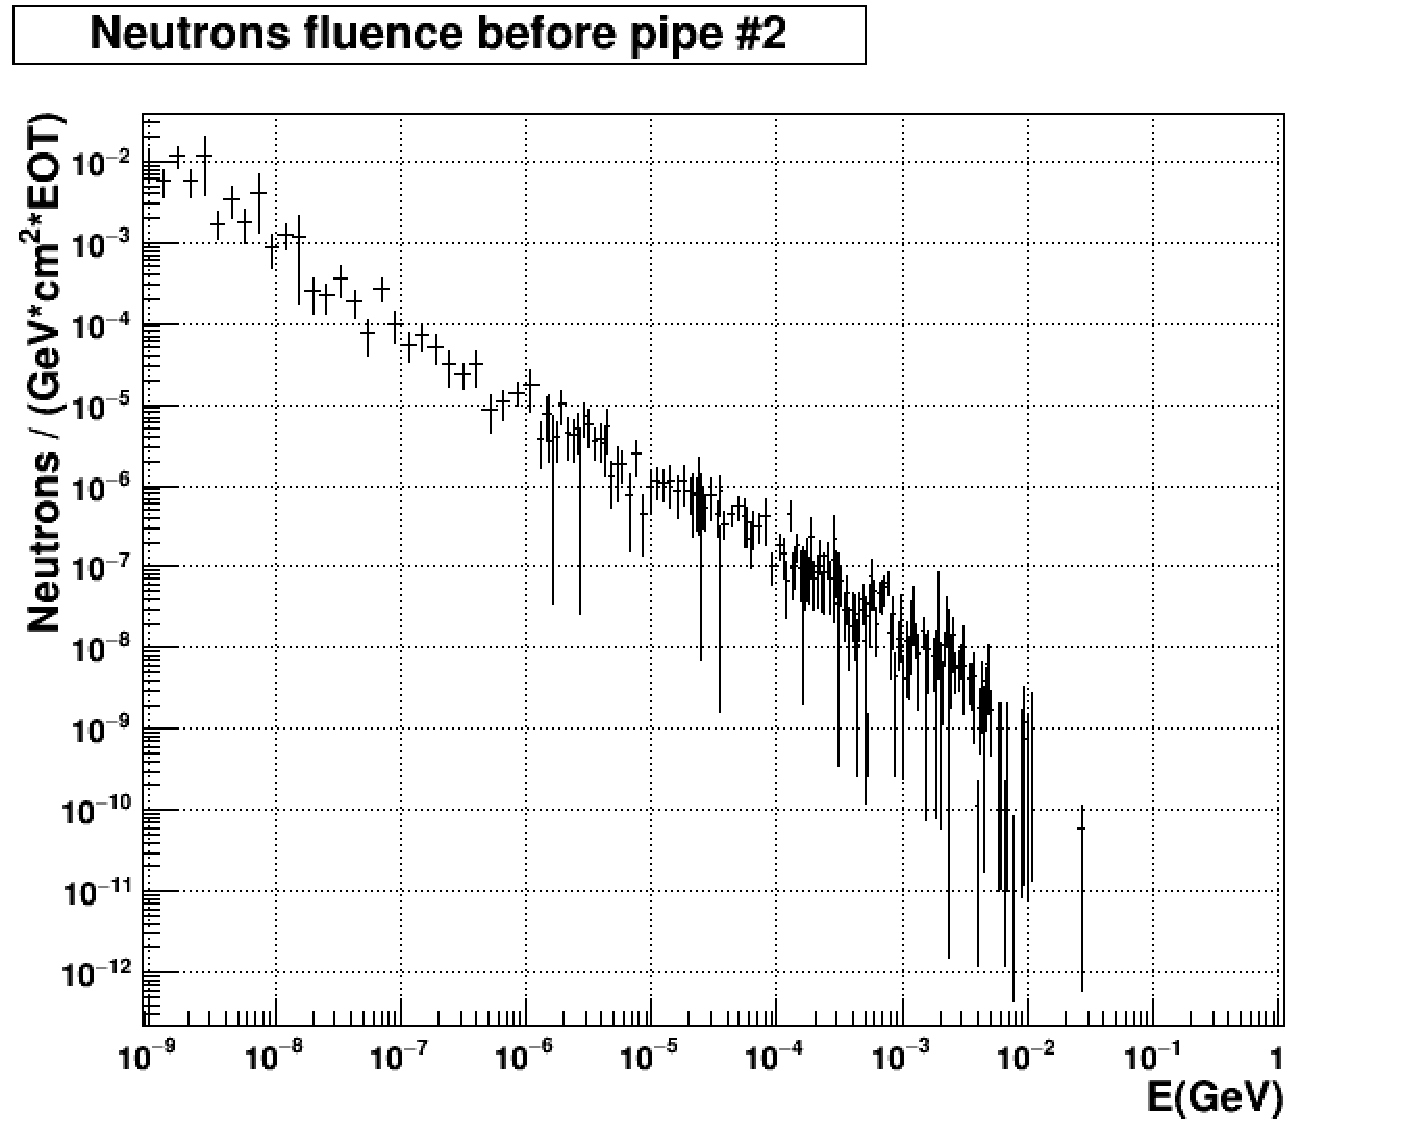
\includegraphics[width=4.7cm]{figs/NeutronsPipe2_1D.pdf}
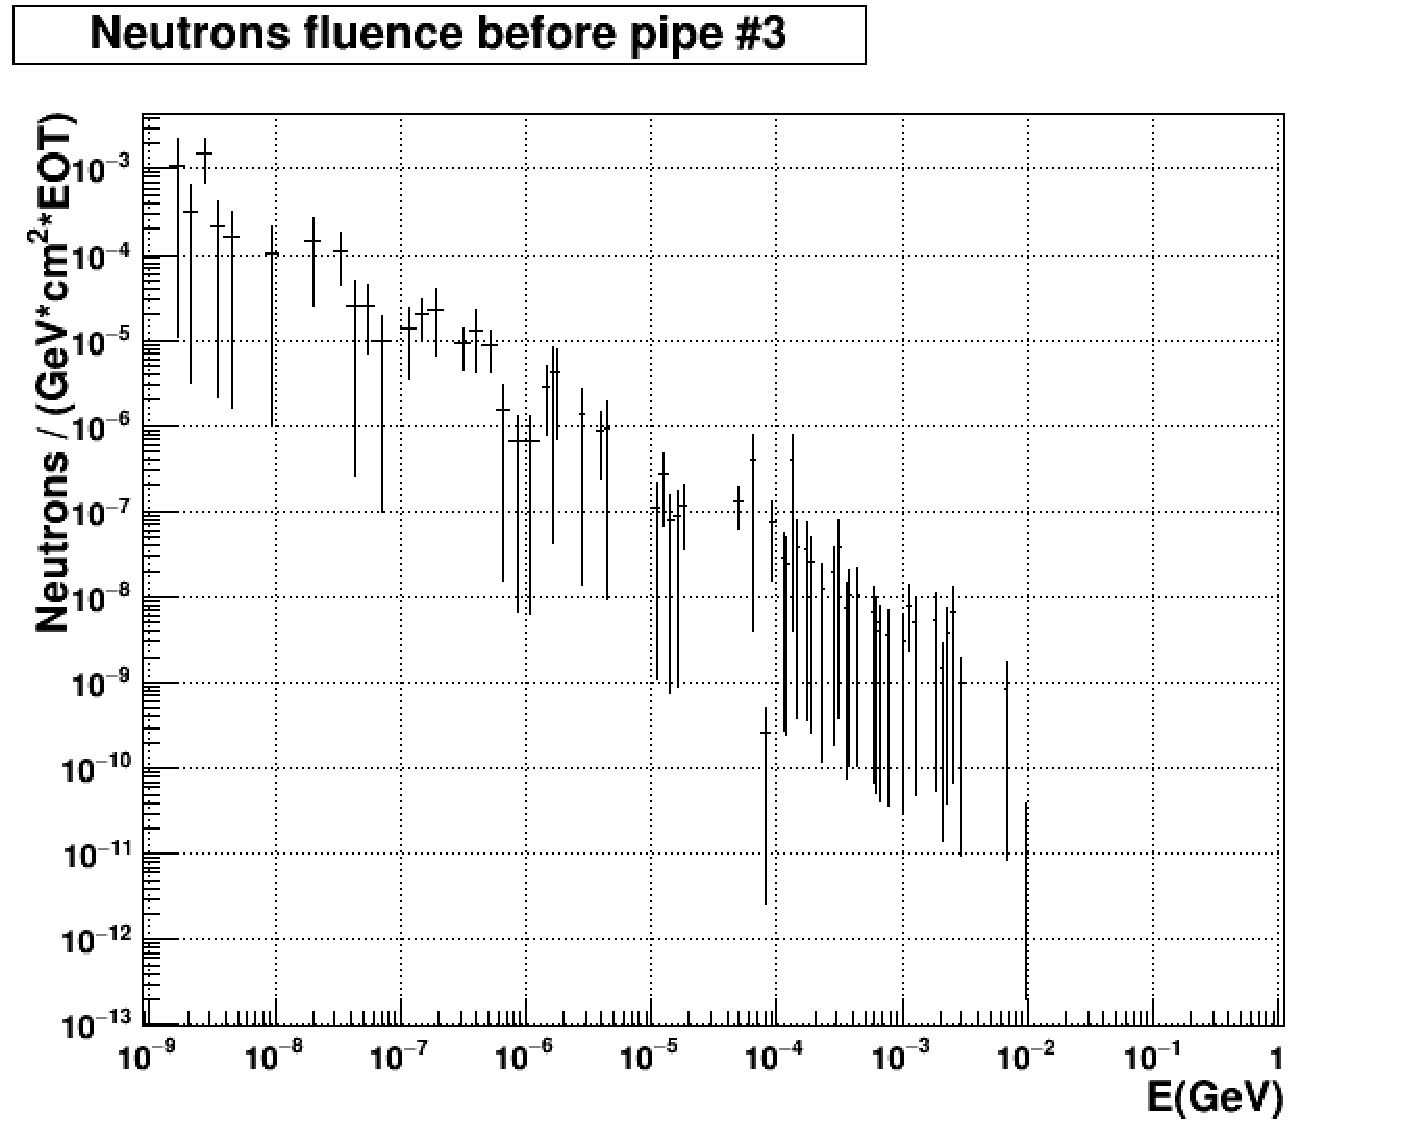
\includegraphics[width=5.5cm]{figs/NeutronsPipe3_1D.pdf}
\caption {Neutron energy spectra at the three locations of interest. Spectra are obtained from electron beam interaction with the beam-dump using FLUKA.}
\label{fig:nu-comp}
\end{figure}


\subsubsection{Cosmic background}

\subsection{The proposed test}

